%! TEX root = **/010-main.tex
% vim: spell spelllang=en:

\section{Performance analysis and optimizations}

\Cref{fig:time_cuda} shows a comparison of the execution time of the initial implementation of the CUDA version against the sequential version for calculation of the diameter of the cycles. For this benchmark, $10^4$ steps were performed on each trajectory. We can observe that the execution time
in CUDA for 1 to $2^{14}$ trajectories is roughly the same but past this point the time starts to increase at a ratio similar to the sequential code.
{\bf why???}


\begin{figure}[H]
    \centering
    \includegraphics[width=1.0\textwidth]{figures/plots/time.tikz}
    \caption{Execution time of CUDA version vs. Sequential \\ (Diameter
    calculation)}%
    \label{fig:time_cuda}
\end{figure}

\begin{figure}[H]
    \centering
    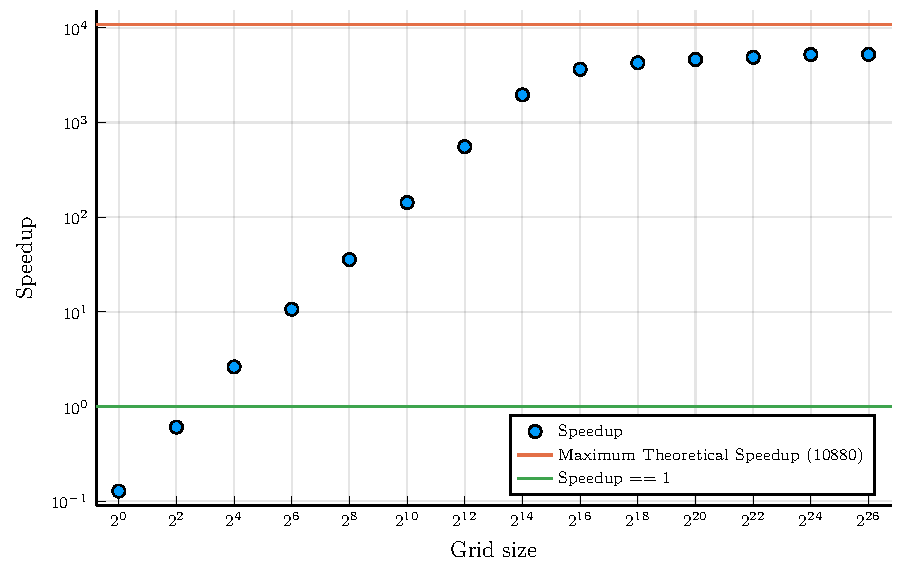
\includegraphics[width=1.0\textwidth]{figures/plots/speedup.tikz}
    \caption{Speedup of CUDA version vs. Sequential \\ (Diameter
    calculation)}%
    \label{fig:speedup}
\end{figure}

{\bf define speedup ???}

The dependence of the speedup on the number of trajectories is shown in \cref{fig:speedup}. 
The overhead for starting CUDA processes make the GPU code slower for calculation of small number of trajectories. For $\approx 2^6 =64$ trajectories the parallel and the serial codes require a similar execution time. The parallel code runs faster (speedup larger than one) for larger number of trajectories. The theoretical maximum for speedup is limited by the number of cores in GPU (10240 in the present case) while here we observe $10^3$ at maximum. There is still an order of magnitude from the maximum achievable speedup which gives room for improvement. Specially if we use additional GPUs. For reference, the computation of $2^{22} \approx 10^6$ trajectories took 4.284s on the GPU while the sequential version of the program takes around 40 minutes.
{\bf ??? check how i changed the text}